\newpage
\section{Particle characterization and particle tracking using interference properties}
		\label{sec:chapter2}

\subsection{Introduction}

Properties of coherent light to produce interference is widely use in metrology for a long time with, for example, the famous Fabry-Pérot  \cite{fabry_theorie_1899, perot_application_1899} and Michelson interferometers \cite{michelson_relative_1887}. The latter was initially used to measure earth's rotation and is still used today, in particular, for the recent measurement of gravitational waves
\cite{ligo_scientific_collaboration_and_virgo_collaboration_gw151226_2016}. 
Since the beginning of the century, interest on tracking and characterizing colloidal particles risen thanks to the democratization of micro fluidics and lab-on-a-chip technologies. In the following I will provide some insights on the three most used :

\begin{itemize}
	\item Reflection Interference Contrast Microscopy (\gls{RICM})
	\item Lorenz-Mie fit
	\item Rayleigh-Sommerfeld back-propagation
\end{itemize}

The first one, \gls{RICM}, uses the principle of optical difference path as a Michelson interferometer. The other two, uses the interference between the light scattered by the colloid and the incident light. Generally, both of the sources  are colinear, thus, speak of in-line holography. 

\subsection{In-line holographic video microscopy theory}

\subsubsection{Reflection Interference Contrast Microscopy}

\begin{figure}[h]
	\centering
	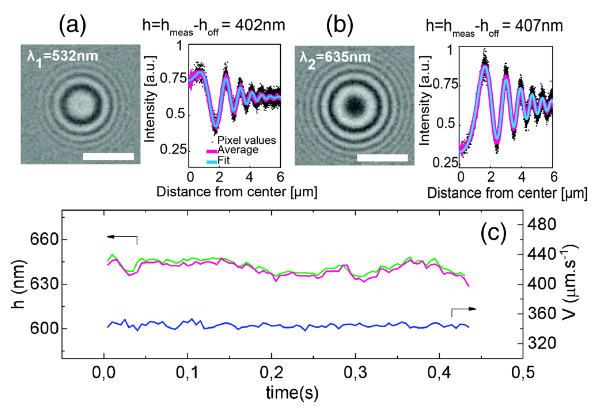
\includegraphics[scale=1]{02_body/chapter2/images/RICM.png}
	\caption{Figure from \cite{davies_elastohydrodynamic_2018} representing \gls{RICM} with two wavelengths. (a) Left: interference patterns created with a wavelength $\lambda_1 = 532$ nm (scale bar $ 5~\mathrm{\mu m}$). 
		Right: radial intensity profile (black dots) extracted from the image, azimuthally averaged (magenta line) and fitted with Eq.\ref{Eq.RICM} to measure the height of the particle (here $h$). (b) Same as (a) with a wavelength $\lambda_2 = 635$ nm. (c) Time series of the height of a particle $h$ (green: $ \lambda_1$, magenta: $\lambda_2$) and the particle velocity measured along the flow in blue. }
	\label{fig.RICM}
\end{figure}


Reflection Interference Contrast Microscopy was first introduced in cell biology by Curtis to study embryonic chick heart fibroblast \cite{curtis_mechanism_1964} in 1964. \gls{RICM} gained in popularity 40 years after both in biology and physics \cite{filler_reflection_2000, siver_use_2000, weber_2_2003, limozin_quantitative_2009, nadal_probing_2002, raedler_measurement_1992}. It was also used recently in soft matter physics to study elastohydrodynamic lift at a soft wall \cite{davies_elastohydrodynamic_2018}.

When we illuminate a colloid with a plane wave from the bottom, a part of the light is reflected at the surface of the glass substrate and at the colloid's surface. The difference of optical path between two reflection create interference patterns. Let's take an interest at the mathematical description of this phenomenon. In the far field, we can describe two different one-dimensional electric field vectors of the same pulsation $\omega$ \cite{f_bohren_absorption_1998} as:

\begin{equation}
	\vec{E}_1(\vec{r}, t) = \vec{E}_{0_1} \cos(\vec{k}_1 \cdot \vec{r} - \omega t + \epsilon_1) ~,
\end{equation}
and
\begin{equation}
	\vec{E}_2(\vec{r}, t) = \vec{E}_{0_2} \cos (\vec{k}_2 \cdot \vec{r} - \omega t + \epsilon_2) ~.
\end{equation}


\nomenclature{$\vec{E}$}{Electrical field}
\nomenclature{$k$}{Wave number}
\nomenclature{$\omega$}{Pulsation}

Where the $k$ is the wave number $k=2\pi n_{\mathrm{m}}/\lambda$, $\lambda$ denoting the illumination wavelength, $n_\mathrm{m}$ the optical index of the medium, $\epsilon_{1,2}$ the initial phase of each wave and $\vec{r}$ the position from the source. Here, the origin ($\vec{r} = \vec{0}$) could be taken at the position of the first reflection (on the glass slide) thus at the particle, $\vec{r}$ would be given by the particle's height such that $|r| = z$ the particle-subtract distance. Experimentally, we measure the intensity of the interference patterns, those can be computed from the time averaged squared sum of the electric field $\vec{E} = \vec{E}_1 + \vec{E}_2$. The measured intensity is thus given by:

\begin{equation}
	\begin{aligned}
		I & = \langle \vec{E}^2 \rangle = \langle \vec{E}_1^2 + \vec{E}_2^2 + 2\vec{E}_1 \cdot \vec{E}_2 \rangle 
		= \langle \vec{E}_1^2 \rangle + \langle \vec{E}_2^2 \rangle  + 2 \langle \vec{E}_1 \cdot \vec{E}_2 \rangle \\
	\end{aligned}
\end{equation} 

where $ \langle \vec{E}_1^2 \rangle $ and  $\langle \vec{E}_2^2 \rangle$ are respectively given by $I_1$ and $I_2$, the incident light intensities. Using the trigonometric formula $2 \cos (a)\cos (b) = \cos (a+b) + \cos (a-b) $ we have:

\begin{equation}
	\langle  
	\vec{E}_1 \cdot \vec{E}_2 \rangle = 
	\langle
	\frac{1}{2} \vec{E}_{0_1}  \vec{E}_{0_2} 
	\left[
		\cos 
		\left(
			\vec{k}_1 \cdot \vec{r} - \vec{k}_1 \cdot \vec{r} + \phi	
		\right)	
		+ 
		\cos
		\left(
			2\omega t + \phi'
		\right)
	\right]
	\rangle~.
\end{equation}

As we average over the time, the second $\cos$ will vanish since in general $\langle \cos(at + b) \rangle_ t = 0$ thus:

\begin{equation}
	\langle \vec{E}_1 \cdot \vec{E}_2 \rangle = \frac{1}{2} \langle  \vec{E}_{0_1}  \vec{E}_{0_2} \rangle
	\cos 
	\left(
	\vec{k}_1 \cdot \vec{r} - \vec{k}_2 \cdot \vec{r} + \phi	
	\right)	
\end{equation}

with $\phi$ the phase difference between the two fields, which is generally equal to $\pi$ due to the reflection properties on a higher index. Indeed, a colloid has generally a greater optical index than the dilution medium.  Finally, the total intensity can be read as:


\begin{equation}
	I = I_1 + I_2 + 2 \sqrt{I_1 I_2} 
	\cos 
	\left(
	\vec{k}_1 \cdot \vec{r} - \vec{k}_2 \cdot \vec{r} + \phi	
	\right)
\end{equation}

By taking $k_1 = - k_2$ due to the reflection properties, we have:


\begin{equation}
	I = I_1 + I_2 + 2 \sqrt{I_1 I_2} 
	\cos 
	\left(
	\frac{4 \pi n_{\mathrm{m}}}{\lambda} z + \phi	
	\right)
\end{equation}


If we now suppose that we have a spherical particle at a height $z$ we can develop the radial interference intensity $I(x)$ as \cite{ raedler_measurement_1992}:

\begin{equation}
	I(x) = A_0 + A_1 \mathrm{e}^{-b_1 x^2} + A_2^{-b_2 x^2} \cos \left[ \frac{4\pi n_m}{\lambda}\left( g(x) + z \right) + \phi \right]
	\label{Eq.RICM}
\end{equation}

Where $A_i$ and $b_i$ are fit parameters and $g(x)$ denotes the contour of the sphere.
Finally, this method is great because the equation is computationally light and permits to have a quick tracking of particles. However, as we can see on Eq.\ref{Eq.RICM}, due to the periodicity of the cosinus, the interference pattern will be the same for all heights $z$ separated by a distance $\lambda / 2n_\mathrm{m} \approx 200 $ nm (for $\lambda = 532$ nm and $n_{\mathrm{m}} = 1.33$). It is possible to extend this limitation by using 2 different wavelength to $\approx 1.2 ~ \mathrm{\mu m}$ as used in \cite{davies_elastohydrodynamic_2018}. Despite the precision of this method which can reach the $10$ nm spatial resolution; the measurement ambiguity is not compatible with the study of  micro-particle Brownian motion, hence, \gls{RICM} is not usable for our context. As a matter of fact, we experimentally reach height span of a few microns. 



\subsubsection{Lorenz-Mie Fit}
\label{chap:LM_fit}

When a colloid is illuminated with a plane wave, a part of the light is scattered. In consequence, the superimposition of the incident field $\vec{E}_0$ and scattered field $\vec{E}_s$ interferes. The interference patterns thus obtained are called holograms. If the particle size is at the same order of magnitude or greater than the illumination wavelength, it is not possible to use Rayleigh approximations \cite{strutt_lviii_1871}. Indeed, we would need to use what we call  the Lorenz-Mie theory which describes the scattering of dielectric spheres; this theory was found by Lorenz and independently by Mie in 1880 and 1908 \cite{lorenz_lysbevaegelsen_1890, mie_beitrage_1908}. 

It is in the early 2000 that the Lorenz-Mie theory was first used in order to track and characterize particles \cite{ovryn_imaging_2000, lee_characterizing_2007}. Since then, a lot of studies has been realized with this method \cite{katz_applications_2010}. In the following I will describe the Lorenz-Mie Fit method.

Let the incident field be a plane wave uniformly polarized along the axis $ \hat{e}$, with an amplitude $E_0$ and propagating along the $z$ direction :
\begin{equation}
	\vec{E}_0(\vec{r},z) = E_0(\vec{r}) \mathrm{e}^{ikz}\hat{e}
\end{equation}

Let's consider a particle of radius $a$ at a position $\vec{r}_p $, the scattered field can be written using the Lorenz-Mie theory \cite{f_bohren_absorption_1998} as:

\begin{equation}
	\vec{E}_s(\vec{r}, z) =  \vec{f}_s(k(\vec{r} - \vec{r}_p))E_0(\vec{r}) \exp \left(-ikz\right) 
\end{equation} 

With $\vec{f}_s$ the Lorenz-Mie scattering function \cite{f_bohren_absorption_1998}. The intensity $I$ that we measure at $\vec{r}$ is given by the superimposition of incident and scattered waves. Since the measurements are done at the focal plane, $I$ is given by:

\begin{equation}
	\begin{aligned}
	I(\vec{r}) & = |\vec{E}_s(\vec{r}, 0) + \vec{E}_0(\vec{r}, 0)|^2 \\
	& = E_0^2(\vec{r}) + 2 E_0^2\operatorname{Re} \left(\vec{f}_s(k(\vec{r}- \vec{r}_p)) \hat{e}\right) + | \vec{f}_s(k(\vec{r}- \vec{r}_p)) |^2
	\end{aligned}
\end{equation}

The most of the experimental defects on the images are due to spacial illumination variation caused by dust particle and such. It can be corrected by normalizing the image by the background. In another word, we normalize  $I(\vec{r})$ by the intensity of the incident field $I_0 = E_0(\vec{r})^2$ which is the experimental background. It can be measured by different methods, one is to have an empty field of view and the other one, which is more convenient is to take the median of a stack of images. Naturally, for having the latter to work, the movie should be long enough to have the particle diffuse enough, if not a ghost of the particle will appear on the background. This process also permits getting rid of the immobile particle that could generate any additional noise. An example of hologram before and after the normalization is shown in Fig.\ref{fig.Lorenz_mie_demo} a-c). We write the normalized intensity $I/I_0$:

\begin{equation}
	\frac{I(\vec{r})}{I_0(\vec{r})} = 1 + 2 \operatorname{Re} 
	\left(  
		\vec{f}_s(k(\vec{r}- \vec{r}_p)) \hat{e}
	\right)
	+
	|
		\vec{f}_s(k(\vec{r}- \vec{r}_p))
	|^2
	\label{Eq.normalized_Mie}	
\end{equation}


Now that we have the analytical form of the holograms' intensity, it is possible to fit an experimental one to Eq.\ref{Eq.normalized_Mie} as shown in Fig.\ref{fig.Lorenz_mie_demo} d-e). For the sake of completeness, I will detail the Lorenz-Mie scattering function, $\vec{f}_s(k\vec{r})$ which is given by the series:

\begin{equation}
	\vec{f}_s(k \vec{r}) = \sum _{n=1} ^{n_c} 
	\frac
	{
		i^n (2n +1)
	}
	{
		n(n+1)
	}
	\left(
		i a_n \vec{N}^{(3)}_{eln}(k\vec{r})
		-
		b_n \vec{M}^{(3)}_{oln}(k\vec{r})
	\right)
	\label{Eq.Lorenz-Mie-function}
\end{equation} 


where $\vec{N}^{(3)}_{eln}(k\vec{r})$ and $\vec{M}^{(3)}_{oln}(k\vec{r})$ are the vector spherical harmonics. $a_n$ and $b_n$ are some coefficients that depend on the particle and illumination properties. For a spherical and isotropic particle of radius $a$ and refractive index $n_\mathrm{p}$, which is illuminated by a linearly polarized plane wave, the $a_n$ and $b_n$ coefficients are expressed in terms of spherical Bessel $j_n$ and Hankel $h_n$ functions as \cite{f_bohren_absorption_1998}:

\begin{equation}
	a_n = 
	\frac
	{
		\zeta^2 j_n (\zeta k a)k a j_n' (k a) - j_n(ka)[\zeta kaj_n(\zeta ka)]'
	}
	{
		\zeta^2 j_n (\zeta k a)k a h_n^{(1)'} (k a) - h_n^{(1)}(ka)\zeta kaj_n'(\zeta ka)
	}
\end{equation}

and

\begin{equation}
	b_n =
	\frac
	{
		j_n(\zeta k a) kaj_n'(ka) - j_n (ka) \zeta kaj_n'(mka)
	}
	{
		j_n(\zeta k a) kah_n^{(1)'}(ka) - h_n^{(1)} (ka) \zeta kaj_n '(mka)
	} ~,
\end{equation}


	where $\zeta = n_\mathrm{p} / n_m$ and the prime notation denotes differentiation with respect to the argument. As we can see, the holograms will depends on Eq.\ref{Eq.Lorenz-Mie-function} and will vary with a lot of parameters ($\lambda$, $n_m$, $n_\mathrm{p}$, $a$ and $\vec{r}_\mathrm{p}$) which can all be fitted. In general, the illumination wavelength $\lambda$ and medium index $n_\mathrm{m}$ are known and do not need to me fitted. From only one hologram it is could thus be possible to measure precisely the position of the particle $\vec{r}_\mathrm{p}$ and in the same time characterize the radius and optical index of the colloid. As a side note, it is even possible to characterize a particle without a priori knowledge of its characteristics using Bayesian approach \cite{gregory_bayesian_2005, dimiduk_bayesian_2016}.

Computing Eq.\ref{Eq.Lorenz-Mie-function} numerically brings another interesting question, as it is analytically written as a sum over $n$; one could ask after which number of terms $n_c$ the series will converge. It has actually been found that the series converge after a number of terms \cite{lentz_generating_1976}
\begin{equation}
	n_c = k a + 4.05 (k a)^{1/3} + 2 ~.
\end{equation}

Consequently, larger particles' holograms will need more terms to converge and, hence, are longer to fit. As an example, the largest particles used during my thesis have a radius $a = 2.5 ~ \mathrm{\mu m}$ leading to a number of terms $ n_c = 55$ in water and $\lambda = 532$ nm, for the smallest ones, where $a = 0.5 ~ \mathrm{\mu m}$ we find $n_c = 18$ which makes a huge difference in practice.

If a reader wants to evaluate an hologram given by the Lorenz-Mie theory for a peculiar particle and position, it can be done in a few lines with the \mintinline{python}{holopy} module using the following Python snippet which was used to make Fig.\ref{fig.holo_fix_n} and \ref{fig.holo_fix_z}:

\begin{minted}
	[
	frame=lines,
	framesep=2mm,
	baselinestretch=1.2,
	fontsize=\footnotesize,
	linenos
	]
	{python}
import holopy as hp
from holopy.scattering import calc_holo, Sphere

sphere = Sphere(n=1.59, r=1.5, center=(4/0.1, 4/0.1, 10))
# n is the optical index of the particle, r it's radius in microns
# center is its center position in microns.

medium_index = 1.33
illum_wavelen = 0.532
illum_polarization = (1, 0)
detector = hp.detector_grid(shape=100, spacing=0.1)
# shape is the size in pixel of the camera and the spacing is the pixel's size in microns.

holo = calc_holo(
	detector, sphere, medium_index, illum_wavelen, illum_polarization, theory="auto"
)
#the hologram can be directly be plotted using:
hp.show(holo)
\end{minted}

\begin{figure}[H]
	\centering
	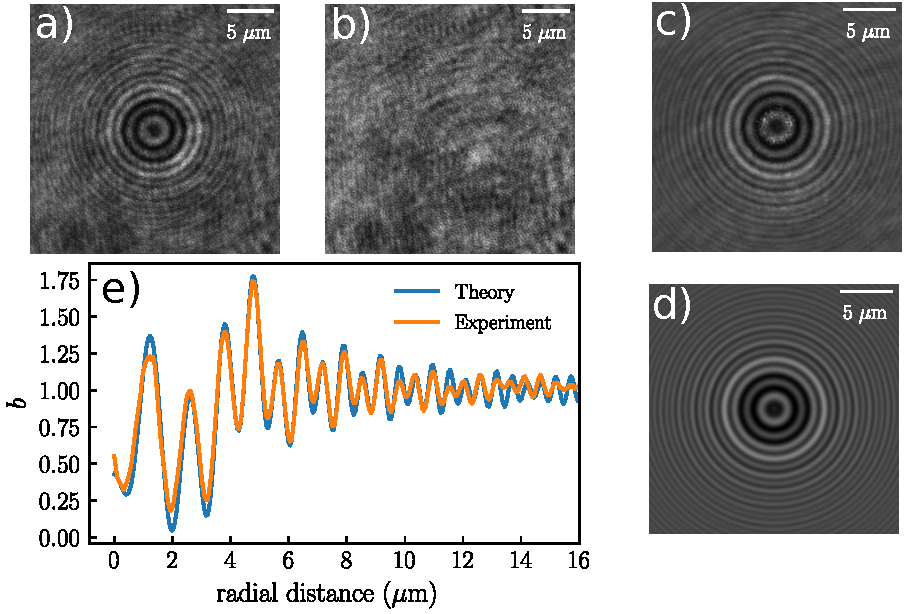
\includegraphics[scale=1]{02_body/chapter2/images/lorenz_mie_fit_demo/plot_lorenz_mie.pdf}
	\caption{a) Raw hologram of a $2.5 ~ \mathrm{\mu m}$ polystyrene particle measured experimentally with the setup detailed in the chapter \ref{chap:exp-setup}. b) Background obtained by taking the median value of the time series of images of the diffusing particle. c) Normalized hologram given by dividing a) by b). d) Result of the fit of c) using Eq.{\ref{Eq.normalized_Mie}} the particle is found to be at a height $z = 14.77 ~ \mathrm{\mu m}$. e) Comparison of the normalized radial intensity, obtained experimentally form c) and theoretically from d).}
	\label{fig.Lorenz_mie_demo}
\end{figure}


In order to know what to experimentally expect, one can to compute holograms for particles of different size and height, as shown in the Fig.\ref{fig.holo_fix_n} with a fixed optical index $n = 1.59$. In this case, one can observe that as $z$ increases, the hologram's rings gets larger. Unlike a Michelson interferometer or \gls{RICM} we do not observe the rings scrolling. Additionally, this thickening of the rings can also be observed on the Fig.\ref{fig:holo_z_fit}, where hologram's intensity profile are plot as a function of the height $z$. Moreover, we can see that the contrast of the holograms are reduced when the height $z$ is small compared to the radius of the particle. Thus, for having an optimal condition for the fits, one should take care to defocus the enough the objective lens to have $z >> a$.


Finally, Lorenz-Mie is the most versatile in-line holographic method, indeed, it permits tracking and characterize unique particles even without a priori knowledge. Besides, it is possible to write the Lorenz-Mie function $\vec{f}_s$ for particular cases such as anisotropic \cite{fung_holographic_2013}, non-spherical particles \cite{wang_using_2014} or particle clusters \cite{fung_holographic_2013, perry_real-space_2013} to name a few; such possibilities open the door to a lot of experimental studies. Additionally, it can reach really high precision as the tenth of nanometer on the position and radius as well as $10^{-3}$ on the optical index \cite{lee_characterizing_2007}. Unfortunately, the Lorenz-Mie fitting suffer from a major drawback which is the time needed to fit one image. For example, a 200 by 200 pixels image, of a $2.5 ~ \mathrm{\mu m}$ particle's hologram, can take up to two minutes to be fitted using a pure and straightforward python algorithm. A lot of work as been done to have faster tracking, such as random-subset fitting \cite{dimiduk_random-subset_2014}, GPU (graphical processing unit) acceleration, machine-learning \cite{yevick_machine-learning_2014, hannel_machine-learning_2018} and deep neural networks \cite{altman_catch_2020}.




\begin{figure}
	\centering
	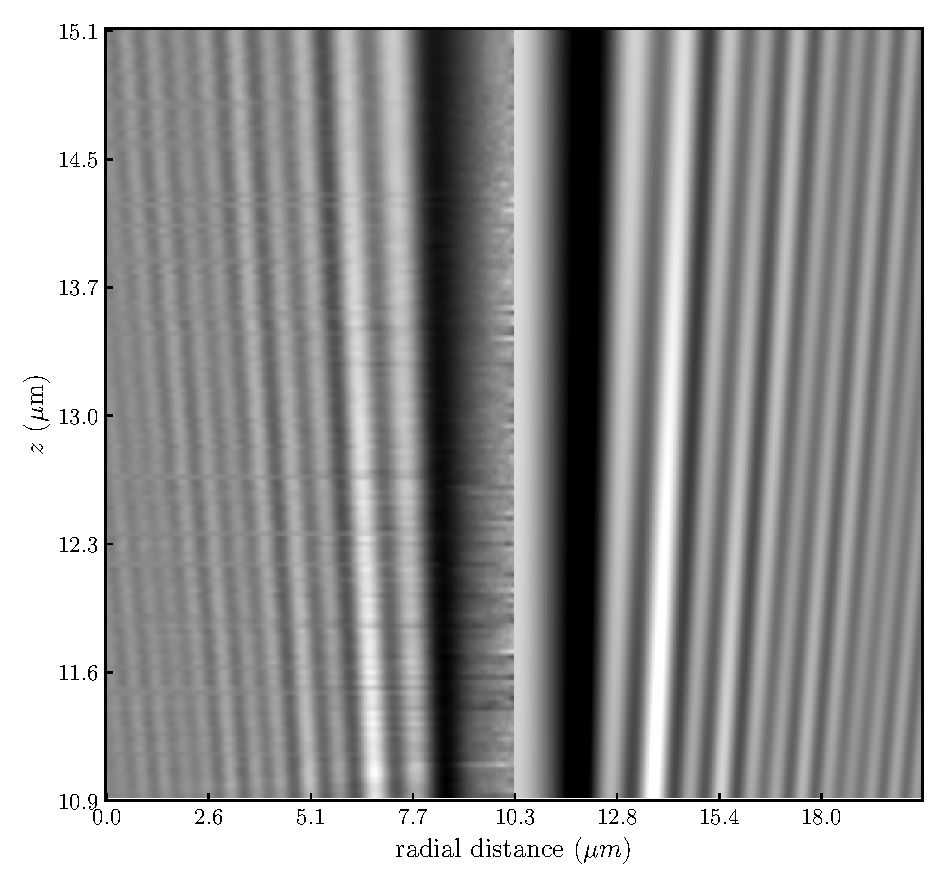
\includegraphics{02_body/chapter2/images/test_tableau2.pdf}
	\caption{On the left, experimentally measured  holograms' radial intensity profile stack, generated from a polystyrene bead of nominal radius $a = 1.5 \pm 0.035 ~ \mathrm{\mu m} $ using the experimental setup explained in chapter \ref{chap:exp-setup}. The calibration of this particle radius and optical index is shown in Fig.\ref{fig:KDErn}. On the right, the corresponding theoretical stack using the result of each individual hologram's fit.}
	\label{fig:holo_z_fit}
\end{figure}



\begin{figure}
	\centering
	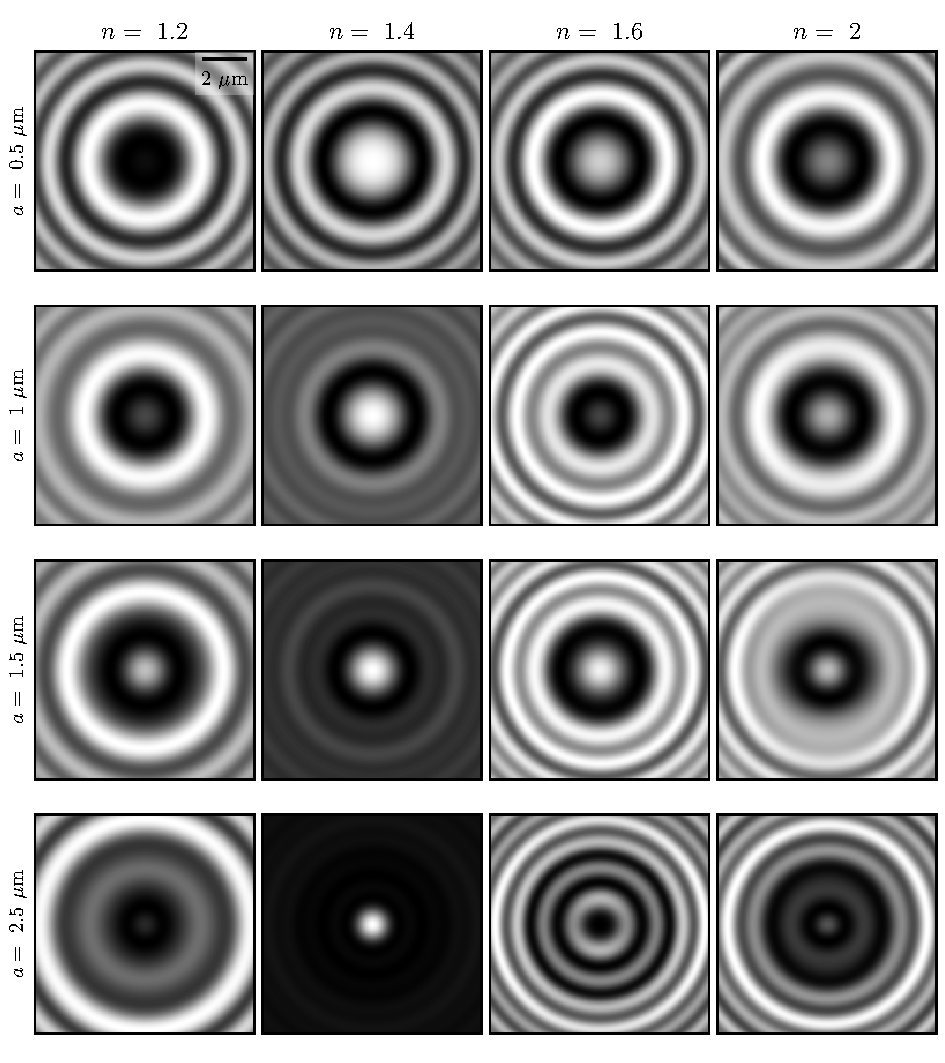
\includegraphics{02_body/chapter2/images/holo_size_exemple/holos_fix_z.pdf}
	\caption{On the left, experimentally measured  holograms' radial intensity profile stack, generated from a polystyrene bead of nominal radius $a = 1.5 \pm 0.035 ~ \mathrm{\mu m} $ using the experimental setup explained in chapter \ref{chap:exp-setup}. The calibration of this particle radius and optical index is shown in Fig.\ref{fig:KDErn}. On the right, the corresponding theoretical stack using the result of each individual hologram's fit.}
	\label{fig.holo_fix_z}
\end{figure}

\begin{figure}
	\centering
	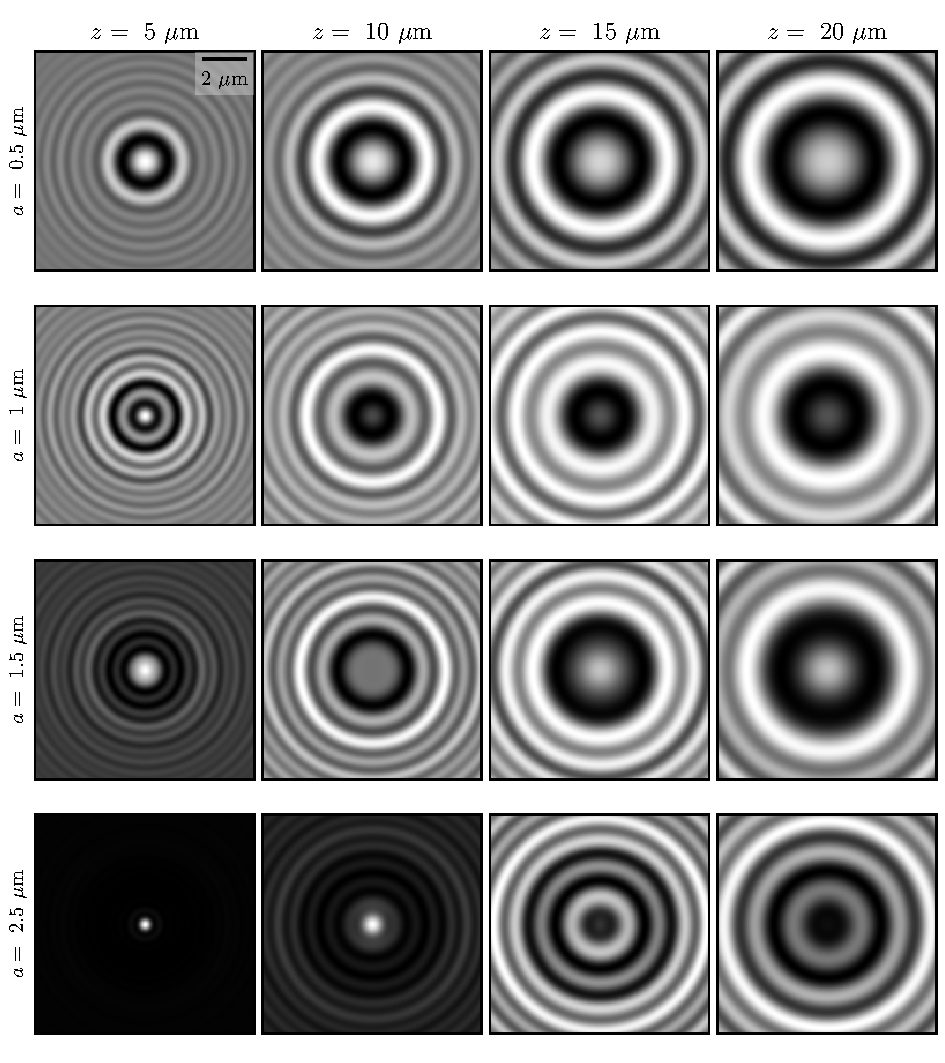
\includegraphics{02_body/chapter2/images/holo_size_exemple/holos_fix_n.pdf}
	\caption{On the left, experimentally measured  holograms' radial intensity profile stack, generated from a polystyrene bead of nominal radius $a = 1.5 \pm 0.035 ~ \mathrm{\mu m} $ using the experimental setup explained in chapter \ref{chap:exp-setup}. The calibration of this particle radius and optical index is shown in Fig.\ref{fig:KDErn}. On the right, the corresponding theoretical stack using the result of each individual hologram's fit.}
	\label{fig.holo_fix_n}
\end{figure}

\newpage

\subsubsection{ Rayleigh-Sommerfeld back-propagation}





Rayleigh-Sommerfeld back-propagation \cite{wilson_3d_2012} works on the same principle as the Lorenz-Mie fitting but assumes that we have small scatterers., such as :

\begin{equation}
	|\zeta - 1| << 1 \text{ and } ka|\zeta - 1| << 1 ~.
\end{equation}

In this case, at the focal plane, the intensity of the scattered field is smaller than the incident field, hence, the term $|\vec{E}_s|^2$ can be ignored. Thus, the normalized intensity, Eq.\ref{Eq.normalized_Mie} can be rewritten as:

\begin{equation}
\frac{I(\vec{r})}{I_0(\vec{r})}= 1 + 2\operatorname{Re}\left( \frac{E_s(\vec{r},0)}{E_0(\vec{r})} \right) ~.
\end{equation}

If one can retrieve completely the scattered field from an image, it is possible to reconstruct it above the focal plane by convolution using the Rayleigh-Sommerfeld propagator \cite{goodman_introduction_2005}:

\begin{equation}
	h_{-z}(\vec{r}) = \frac{1}{2 \pi} \frac{\partial}{\partial z} \frac{\mathrm{e}^{ikR}}{R} ~,
	\label{Eq:propagator}
\end{equation}

where $ R^2 = r^2 + z^2 $ and the sign convention on the propagator indicates if the particle is below or above the focal plane. Using this propagator we have:

\begin{equation}
	E_s(\vec{r}, z) = E_z(\vec{r}, 0) \otimes h_{-z}(\vec{r})
\end{equation}

By using the convolution theorem \cite{cheong_strategies_2010, goodman_introduction_2005, sherman_application_1967,schnars_digital_1994} and supposing a uniform illumination, one can write the reconstructed scattered field at a height $z$ as:

\begin{equation}
	E_s(\vec{r}, z) \approx \frac{\mathrm{e}^{ikz}}{4\pi ^2}
	\int ^\infty _{- \infty}
	B(\vec{q}) H(\vec{q}, -z) \mathrm{e}^{i \vec{q} \cdot \vec{r}} d^2 q
	\label{Eq.RS} ~,
\end{equation}

where $B(\vec{q})$ is the Fourier transform of $I/I_0$ and $H(\vec{q}, -z)$ is given by

\begin{equation}
	H(\vec{q}, -z) = \mathrm{e}^{iz \sqrt{k^2 - q^2}} ~.
\end{equation}

Finally, using Eq.\ref{Eq.RS} one can reconstruct the scattered field and intensity since $I(\vec{r}) = |E_s(\vec{r})|^2$ as shown in Fig.\ref{fig.sommerfeld}. Moreover, by finding the position where the field is the brightest as shown in red the Fig.\ref{fig.sommerfeld}, we measure the position of the particle.
Those equations are way less computational intensive than the Lorenz-Mie function Eq.\ref{Eq.Lorenz-Mie-function}. Thus tracking can be way faster, moreover, Fourier transforms can be largely accelerated using GPU. Additionally, as the propagator Eq.\ref{Eq:propagator} take only into account the intensity of the image, this method does not require any information on the particle and number of particles. As a matter of fact,   to write Eq.\ref{Eq.RS} one just need to assume that we have spherical colloids. Thus, this method is great to reconstruct the 3D position of a lot of particles or clusters formations. However, the major drawback is that it is the less precise of the presented measurements and that we can't use it to characterize the particles generating the holograms.

\begin{figure}[!ht]
	\centering
	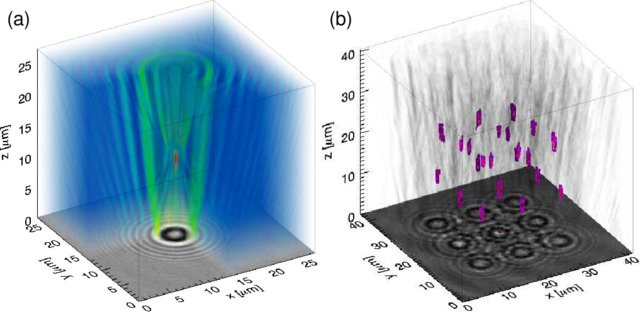
\includegraphics[scale=2]{02_body/chapter2/images/sommerfel_demo.jpg}
	\caption{Figure from \cite{cheong_strategies_2010} a) Volumetric reconstruction using Eq.\ref{Eq.RS} of the scattered intensity of single colloidal sphere, colored by intensity. b) Volumetric reconstructions of $22$ individual $1.58 ~ \mathrm{\mu m}$ diameter silica spheres organized in bcc lattice using holographic optical tweezers in distilled water. Colored regions indicate the isosurface of the brightest 1 percent of reconstructed voxels.}
	\label{fig.sommerfeld}
\end{figure}



\subsubsection{Conclusion}

Finally, the method we choose is the Lorenz-Mie fitting method, since this it permits the characterization of single particles. Indeed, since we are interested to fine effects near the surface, we need to know perfectly the radius of the particle we have recorded. This feature also make our all process calibration free, as we don't need to assume any physical properties. In the following, the experimental setup is going to be detailed.


\subsection{Experimental setup}
\label{chap:exp-setup}
In order to observe the holograms we use an homemade inverted microscope as shown on the Fig.\ref{fig:picture} and shematized in Fig.\ref{fig:schema}. A sample consists of a parallelepipedic chamber ($1.5 ~ \text{cm} ~ \times ~ 1.5 ~ \text{cm} ~ \times ~ 150 ~ \mathrm{\mu m} $), made from two glass covers, a parafilm spacer, and sealed with vacuum grease, containing a dilute suspension of spherical polystyrene beads. We used 3 different sizes, of nominal radii $0.56 ~ \mathrm{\mu m}, ~ 1.5 ~ \mathrm{\mu m} \text{ and } 2.5 ~ \mathrm{\mu m} $, at room temperature $T$, in distilled water (type 1, MilliQ device) of viscosity $\eta = 1 ~ \mathrm{mPa.s}$. The sample is illuminated by a collimated laser beam with a $521 ~ \mathrm{\mu m}$ wavelength. As depicted in the chapter \ref{chap:LM_fit}, the light scattered by one colloidal particle at a given time $t$ interferes with the incident beam. An oil-immersion objective lens (x60 magnification, $1.30$ numerical aperture) collects the resulting instantaneous interference pattern, and relays it to a camera (Basler acA1920-155um) with a $51.6$ nm/pixel resolution (see Fig.\ref{fig.Lorenz_mie_demo}a)). The exposure time of the camera is set to $\tau_{\mathrm{expo}} = 3$ ms to avoid motion-induced blurring of the image, as a general rule, the particle should not diffuse more than the pixel size during that time such that here $2D\tau_{\mathrm{expo}} < 51.6$ nm.

\begin{figure}[!ht]
	\centering
	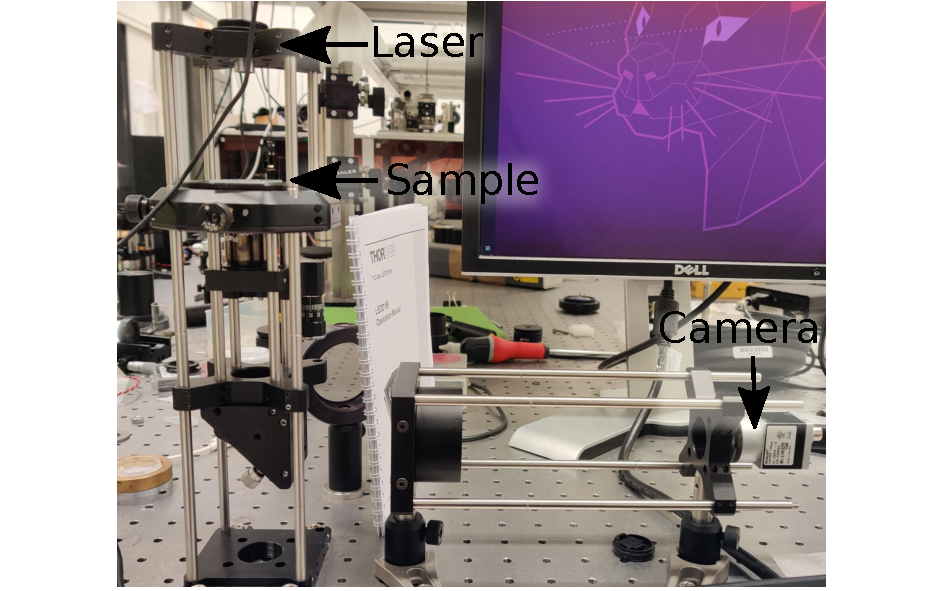
\includegraphics{02_body/chapter2/images/figures_setup/photo_setup.pdf}
	\caption{Photo of the custom build microscope used along my thesis. It is mainly composed of Thorlabs cage system. The camera used is a Basler acA1920-155um, we use a x60 magnification and $1.30$ numerical aperture oil-immersion objective lens. The light source is a colimated  $521 ~ \mathrm{\mu m}$ wavelength laser.}
	\label{fig:picture}
\end{figure}

\begin{figure}[!ht]
	\centering
	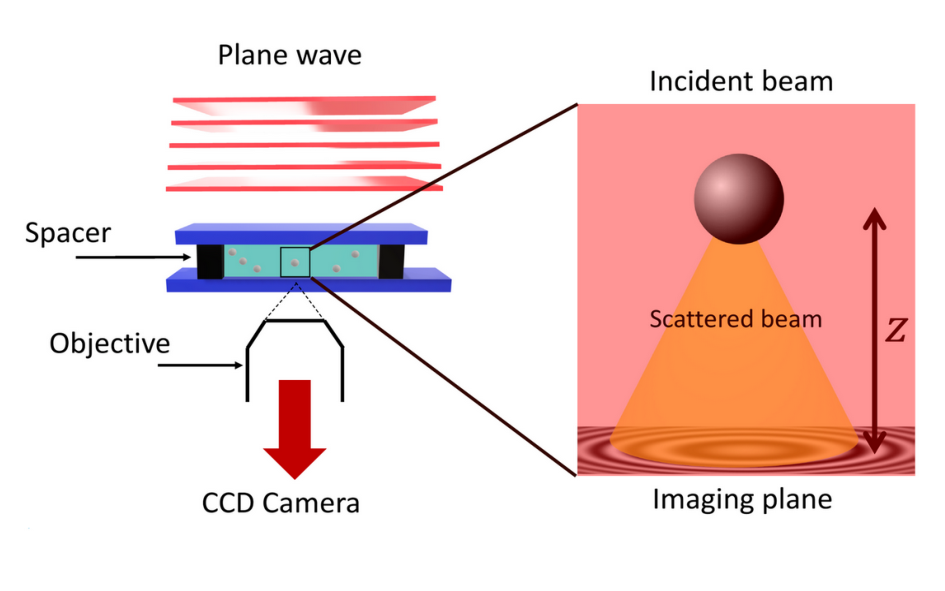
\includegraphics[scale=0.9]{02_body/chapter2/images/figures_setup/schema_setup.pdf}
	\caption{Schematic of the experimental setup. A laser plane wave of intensity $I_0$ illuminates the chamber containing a dilute suspension of micro-spheres in water. The light scattered by a particle interferes with the incident beam onto the focal plane of an objective lens, that magnifies the interference patten and relays it to a camera.}
	\label{fig:schema}
\end{figure}


\subsection{Hologram fitting strategy}

\subsubsection{How to fasten the process ?}

As presented in the section \ref{chap:LM_fit} about the Lorenz-Mie fitting, the main drawback is the time to fit an image, from $30$ seconds for the images of $100 \times  100$ pixels to a few minutes for the $500\times 500$ pixels. We can directly see a bottleneck, indeed, if we want to track one trajectory made of $100~000$ images we would need to wait a minimum of $\approx 70$ days; for a series of images that need only a few minutes to be shot experimentaly. When I started my PhD, two groups, the Grier's lab and the Manoharan's lab, had already introduced python packages, respectively, Pylorenzmie and Holopy in order to inverse holograms. They had introduced ways to only fit a set of randomly chosen pixels, and demonstrated that taking only $1\%$ of the image pixels, could lead to similar precision and improve considerably the fit's execution time \cite{dimiduk_random-subset_2014}. Unfortunately, even if this is faster, it leads to a few images per second and still is too long for the amount of data we wanted to have. Ironically, this part of my project is certainly the one where I spent the most my time, and I actually learned a lot of things on code optimization and computer cluster usage. It's around the half of my thesis, that Pylorenzmie got a new commit on their github repository which was telling that they succeeded on using GPU acceleration using CUDA. This was not an easy task since they needed to reconstruct the Bessel functions in an understandable way for the GPU, fortunately it is possible to do so by using continued fractions \cite{lentz_generating_1976}. This humongous update permits fitting whole images at a whooping speed improvement of 20 fps. At this speed, we fit the tridimension position of the particle, the radius and optical index. To have a more reliable and fast tracking, what we do is that we fit with all free parameters the first $10~000$ images of a movie. We then determine the physical properties of the colloidal particle and then fit the whole movie with only the position as a free parameter.

\subsubsection{Radius and optical index characterization}


Once the data of the radius and optical index retrieved, the quantity we can look at is the the distribution of measurements. Using $10 ~ 000$ measurements we can plot the histograms of the measured $a$ and $n_\mathrm{p}$.




This simple histogram could suffice to measure the physical properties of the colloidal particle. However, we can go a bit further and look at the 2D histogram of the $a$ and $n_\mathrm{p}$ as presented in the fig.\ref{fig:KDErn} here smoothed using a Gaussian kernel density estimator. As we can see it is not isotropic, and it seems that the measurement of $n_\mathrm{p}$ and $a$ are correlated.
 

\begin{figure}[!ht]
	\centering
	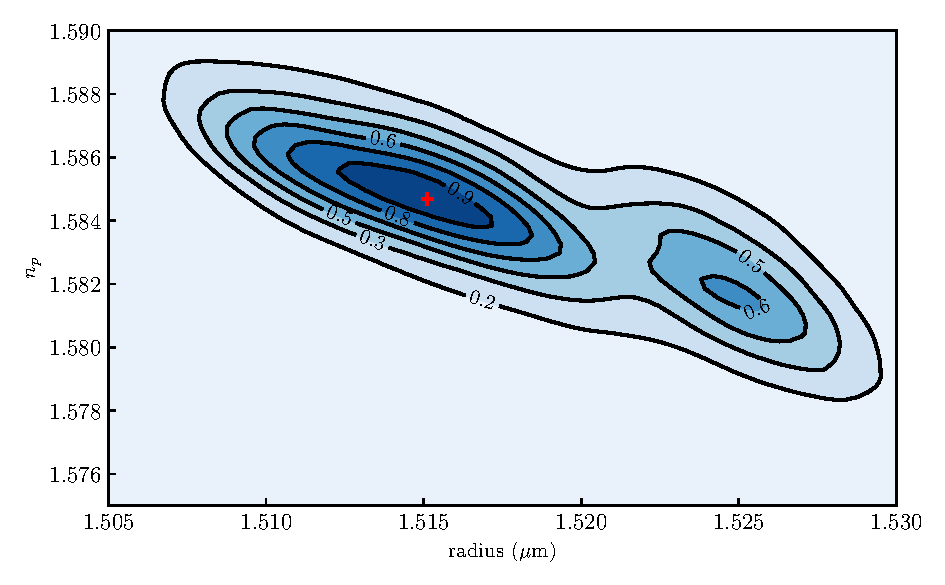
\includegraphics{02_body/chapter2/images/KDErn.pdf}
	\caption{2D Probability density function of the measurements of the optical index $n_\mathrm{p}$ and radius $a$. Black lines indicate iso-probability. Taking the $10\% $ top probability, we measure $n_\mathrm{p} = 1.585 \pm 0.002$ and $a=1.514 \pm 0.003 ~ \mathrm{\mu m}$. }
	\label{fig:KDErn}
\end{figure}